We implemented \sys's programming and execution model as a runtime library and API that a programmer can use to make a plain C program intermittence-safe using \sys.

\subsection{Application Programming Interface}
\label{sec:coala_api}

Coala's API adds only five syntactic constructs to a C-based language, summarized
in Table~\ref{table:coala_api}.
\texttt{COALA\_TASK} is a function annotation that declares a function to be a
task. \texttt{COALA\_NEXT\_TASK}, indicates the task to run next, after an
executing task completes.  \texttt{COALA\_PV} declare a new protected variable.
The programmer uses \texttt{RP} and \texttt{WP}, to read and write protected
respectively.  \texttt{COALA\_SM} identifies protected \texttt{struct} fields
and tells \sys to ensure that the struct fields are page-aligned in memory.
The programmer is required to explicitly call two API functions at the start of
{\tt main()}: \texttt{COALA\_INIT}, which does global initialization upon first
boot and \texttt{COALA\_RUN} which hands the control to \sys's task manager to
resume task execution.

\begin{table}
\centering
\begin{tabular}{| r | p{0.7\columnwidth} |}
	\hline
	{Method} & {Arguments} \\
	\hline\hline
	\texttt{COALA\_INIT}($t$) & $t \in \mathbf{T}$: task to be scheduled on the first boot \\
	\hline
	\texttt{COALA\_RUN}() & --- \\
	\hline
	\texttt{COALA\_TASK}($t$, $w_t$) & $t \in \mathbf{T}$: new task name, $w_t$: weight of task $t$ \\
	\hline
	\texttt{COALA\_NEXT\_TASK}($t$) & $t \in \mathbf{T}$ : task to be run next \\
	\hline
	\texttt{COALA\_PV}($p$, $v$ [, $s$]) & $p$: variable type, $v \in \mathbf{V}$: new protected variable name, $s$: array size \\
	\hline
	$u$ := \texttt{RP}($v$) & $v \in \mathbf{V}$: protected variable to be read, $u$: destination operand \\
	\hline	
	\texttt{WP}($v$) := $u$ &  $v \in \mathbf{V}$: protected variable to be written, $u$: source operand \\
	\hline
	\texttt{COALA\_SM}($p$, $m$ [, $s$]) & $p$: \texttt{struct} member's type, $m$: \texttt{struct} member's name, $s$: array size \\
	\hline
\end{tabular}
\caption{API summary; $\mathbf{T}$: set of all tasks, $\mathbf{V}$: set of all protected variables, $[, s]$: optional argument.}
\label{table:coala_api}
\end{table}

\subsection{API Details}

\textbf{New Tasks.} The \texttt{COALA\_TASK} annotation on a function
declaration statically allocates a non-volatile constant variable holding a
task's weight and declares that the function is a task.

\textbf{Task Transitions.} A call to \texttt{COALA\_NEXT\_TASK} immediately
transfers control to a specified next task and can be invoked along
any control path to dynamically determine the next task.
Like prior work~\cite{chain,dino,ratchet}, \sys's control-flow model
assumes that an executing task is not interruptible by asynchronous events.  

\textbf{Protected Variables.} The \texttt{COALA\_PV} annotation on a
variable statically allocates and aligns a protected non-volatile variable. The
variable must then be accessed with the \texttt{RP} and \texttt{WP} API methods at
runtime to ensure correct operation.

\textbf{Protected Reads and Writes.} The programmer uses the \texttt{RP} and \texttt{WP} API
methods to access protected variables.  These methods cause \sys to find a variable's page.
If the page is not resident in working memory, the method leads to a page fault,
which fetches the page from non-volatile memory. Unlike \texttt{RP},
\texttt{WP} marks the variable's page as dirty, allowing for efficient 
commit back to non-volatile memory. 

\textbf{Initialization.} The behavior of the API method
\texttt{COALA\_INIT} is very similar to \texttt{COALA\_NEXT\_TASK}, with the
addition that all the preliminary kernel initializations are performed inside
this function. 

%\begin{wrapfigure}{t!}{0.5\textwidth}
%	\centering
%	%\includegraphics[width=0.5\columnwidth]{figures/graffle/state-machine.pdf}
%	\caption{\sys state machine implementation \todo{Draw a figure}{Sinan, Carlo}}
%	\label{fig:coala_state_machine}
%\end{wrapfigure}

%A high-level state machine of the execution manager is depicted in Figure~\ref{fig:coala_state_machine} \todo{Draw a figure reflecting the following description}{Sinan, Carlo}. 

\textbf{Execution.} The programmer passes control to \sys's task scheduler 
by calling \texttt{COALA\_RUN} after device initialization. 
%
First the scheduler updates the coalescing target using the coalescing
strategy.  Second, the scheduler resumes a commit, if one is in progress. Third,
the scheduler clears the list of dirty shadow pages. The scheduler then 
sets the program counter to the next task to run, which \sys tracks in  
non-volatile memory.  
%
Before executing the task, \sys checks whether there is a partially committed
task to resume, which requires \sys to restore volatile state, including the program
counter.  
%
If there is no in-progress, partially committed task, \sys starts executing and
coalescing tasks. 
%\todo{Go over keywords (coalescing target, current budget, commit phases etc.) and make them consistent with the rest of the paper}{Amjad, Carlo}

\subsection{Paging}
\label{sec:impl:paging}

As described in Section~\ref{sec:memory_virtulaization}, \sys's memory
virtualization scheme uses three buffers: a volatile \texttt{working} buffer, a
non-volatile main memory \texttt{\underline{store}}, and a non-volatile
\texttt{\underline{shadow}} page buffer. 
%
The main memory \texttt{\underline{store}} holds the last committed copy of all 
pages. 
%
After reboot, the \texttt{working} buffer is empty. Execution fills 
the working buffer with pages as the program accesses them. 
%
The program primarily reads and writes data paged into the volatile working memory. 
%
The non-volatile \texttt{\underline{shadow}} buffer serves as an intermediate,
non-volatile backing store for dirty pages evicted from the space-constrained
working buffer. 

To access a protected variable with either \texttt{RP}
or \texttt{WP}, \sys searches for the variable in its working buffer first. If
found, the program accesses the data in the working buffer.  If the page is not 
in the working memory, the memory manager fetches it from non-volatile memory. 
%
\sys uses address-based page tagging to make finding a variable efficient.  The
upper bits of a variable's memory address identify its page, and the lower bits
denote the variable's offset in its page. The total number of pages in memory,
$p$, determines the number of tag bits, which is $\log P$.

Page tagging imposes a data alignment requirement.
Page size $S$ must be a power of two. 
%
Pages must be aligned to an $S$-byte boundary. 
%
We experimented with 32-, 64-, 128- and 256-byte pages, an 8kB non-volatile \texttt{\underline{shadow}} buffer and
an 8kB non-volatile \texttt{\underline{store}}, and a volatile working buffer
of 1kB, which is half of the total SRAM size in the MSP430FR6989 microcontroller.
%\begin{figure}
%	\centering
%	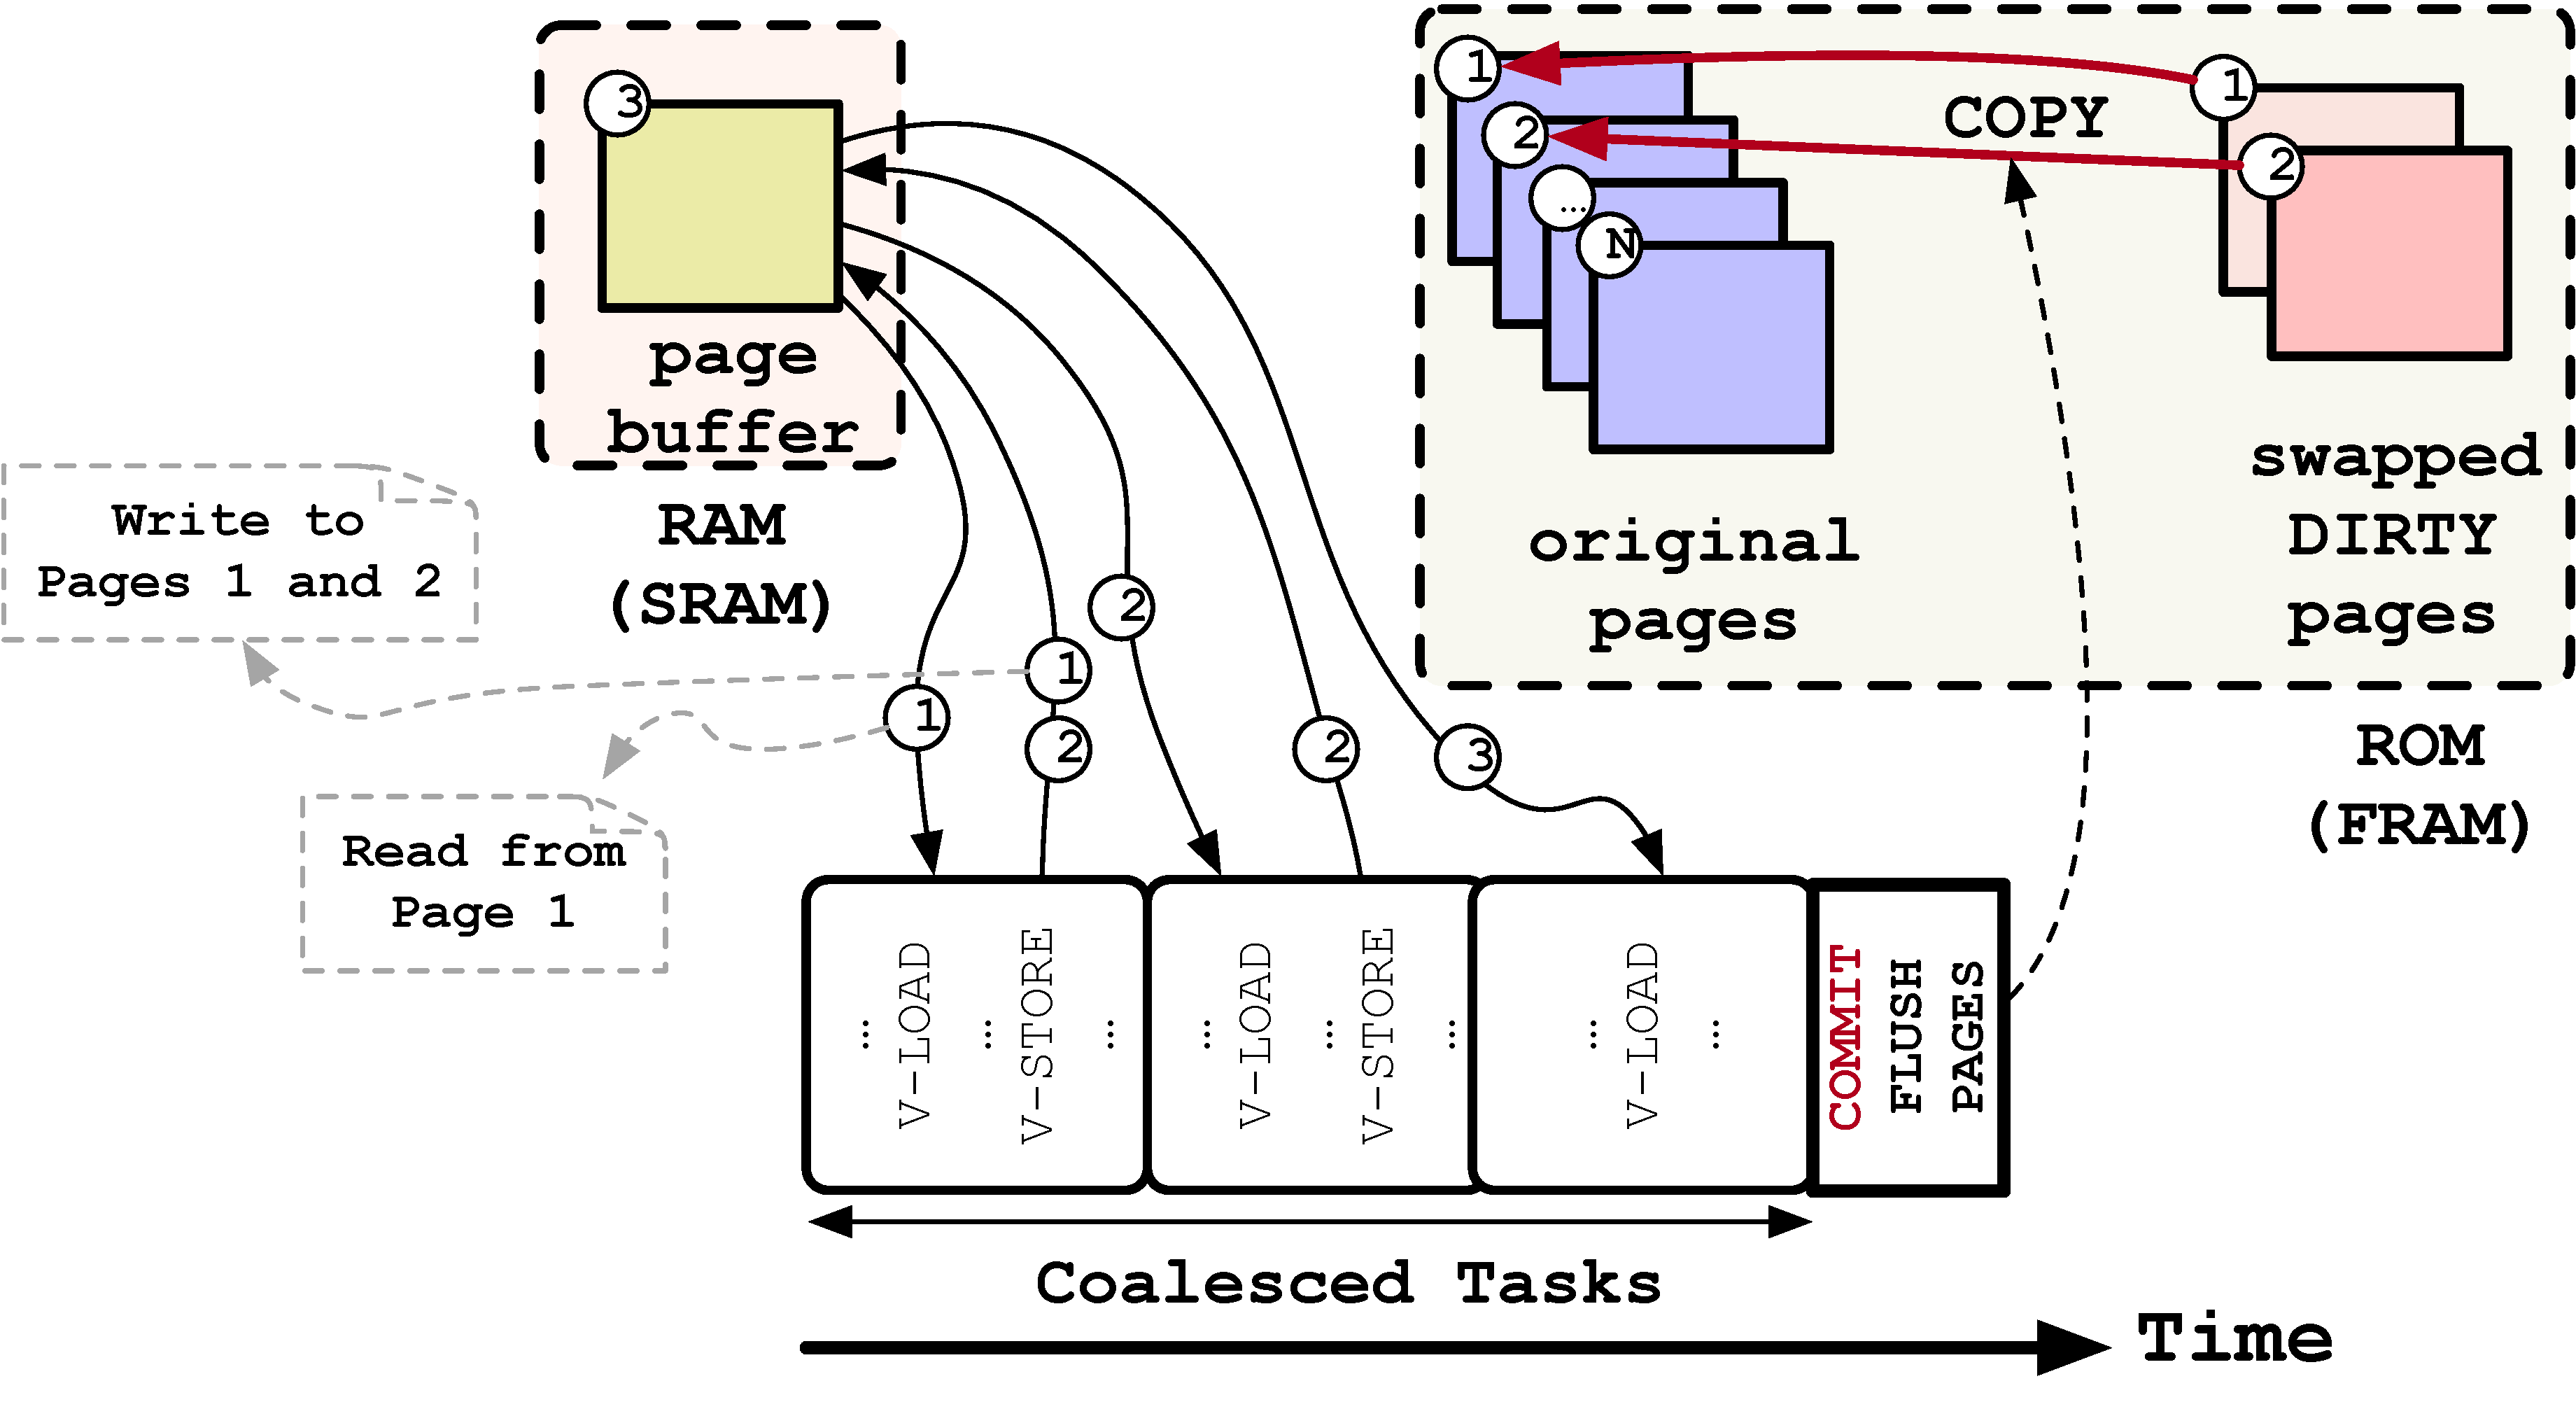
\includegraphics[width=\textwidth]{figures/graffle/paging.pdf}
%	\caption{Illustration of \sys page tags mechanism.}
%	\label{figure:coala_page_tags}
%\end{figure}

% It is important to mention that store and shadow buffers are virtual. By default, \sys allocates two memory banks for pages, $B0$ and $B1$, and all the pages have their store copy in $B0$. A dirty page that during the intermediate commit, or due to eviction, is copied to its shadow location in $B1$, will end up having its store location in $B1$ after the ultimate commit. Thus, during the ultimate commit

\subsection{Coalescing and Commit}


\sys uses a two-phase commit process to atomically commit pages despite
possible power interruptions during commit.  When a coalesced task completes,
\sys backs up dirty pages in volatile working memory to the non-volatile
shadow buffer using DMA. 
%
If power fails while backing up these pages, commit fails and the execution
resumes from the last committed point.  After backing up pages from working
memory to the shadow buffer, \sys sets a flag that indicates an on-going atomic
commit.  At this point, commit is irrevocable and will continue until it
completes despite power failures.   
%
Each page is double buffered, with one copy always in the shadow page buffer
and one copy always in the main memory store.  \sys uses double buffering to
commit dirty pages efficiently by swapping which buffer is which, without
copying any data.
%

\subsection{Task Downscaling}

\sys's task downscaling preserves forward progress by partially committing an
ongoing, non-terminating task. 
%
Partial commit relies on the existence of a hardware timer, which is a very
common feature in a typical MCU and consumes very little energy (i.e.,
$\approx$3\,$\mu$A/MHz~\cite{msp430datasheet}).  

 \textbf{Partial Commit and Task Atomicity.} Some applications prevent
downscaling a task because of a need for task atomicity.  For example, sampling
an analog signal requires consecutive samples at a known interval, or the
digitally sampled signal is meaningless.  In such a case, the programmer can
disable partial commit for a task or a span of code, marking  the code with a
pair of \texttt{COALA\_DISABLE\_PE} and \texttt{COALA\_ENABLE\_PE} annotations.
These annotations respectively halt and resume the partial execution timer.

%\begin{wrapfigure}{t!}{0.5\textwidth}
%	\centering
%	%\includegraphics[width=0.5\columnwidth]{figures/graffle/commits-illustration.pdf}
%	\caption{Intermediate commit and ultimate commit Illustration \todo{to be drawn}{sinan}}
%	\label{fig:intermediate_ultimate-commit}
%\end{wrapfigure}
